% Opcje klasy 'iithesis' opisane są w komentarzach w pliku klasy. Za ich pomocą
% ustawia się przede wszystkim język i rodzaj (lic/inz/mgr) pracy, oraz czy na
% drugiej stronie pracy ma być składany wzór oświadczenia o autorskim wykonaniu.
\documentclass[declaration,shortabstract,mgr]{iithesis}

\usepackage[utf8]{inputenc}

%%%%% DANE DO STRONY TYTUŁOWEJ
% Niezależnie od języka pracy wybranego w opcjach klasy, tytuł i streszczenie
% pracy należy podać zarówno w języku polskim, jak i angielskim.
% Pamiętaj o mądrym (zgodnym z logicznym rozbiorem zdania oraz estetyka) ręcznym
% złamaniu wierszy w temacie pracy, zwłaszcza tego w języku pracy. Użyj do tego
% polecenia \fmlinebreak.
\polishtitle    {Wykrywanie i śledzenie komórek glistopodobnych w programie ImageJ}
\englishtitle   {Worm-like cell detection and tracking in ImageJ}
\polishabstract {Polskie streszczenie}
\englishabstract{English abstract}
% w pracach wielu autorów nazwiska można oddzielić poleceniem \and
\author         {Artur Rosa}
% w przypadku kilku promotorów, lub konieczności podania ich afiliacji, linie
% w poniższym poleceniu można złamać poleceniem \fmlinebreak
\advisor        {dr Andrzej Łukaszewski}
%\date          {}                     % Data złożenia pracy
% Dane do oświadczenia o autorskim wykonaniu
%\transcriptnum {}                     % Numer indeksu
%\advisorgen    {dr. Jana Kowalskiego} % Nazwisko promotora w dopełniaczu
%%%%%

%%%%% WLASNE DODATKOWE PAKIETY
%
%\usepackage{graphicx,listings,amsmath,amssymb,amsthm,amsfonts,tikz}
%
%%%%% WŁASNE DEFINICJE I POLECENIA
%
%\theoremstyle{definition} \newtheorem{definition}{Definition}[chapter]
%\theoremstyle{remark} \newtheorem{remark}[definition]{Observation}
%\theoremstyle{plain} \newtheorem{theorem}[definition]{Theorem}
%\theoremstyle{plain} \newtheorem{lemma}[definition]{Lemma}
%\renewcommand \qedsymbol {\ensuremath{\square}}
% ...

\usepackage{algorithmic,amsmath,graphicx}
\DeclareMathOperator*{\argmax}{\textbf{argmax}}
\newcommand{\image}{\mathbf{I}}
\renewcommand{\algorithmicforall}{\textbf{for each}}

%%%%%

\begin{document}


%%%%%%%%%%%%%%%%%%%%%%%%%%%%%%%%%%%%%%%%%%%%%%%%%%%%%%%%%%%%%%%%%%%%%%%%%%%%%%%%%%%%%%%%%%%
%%%%% POCZĄTEK ZASADNICZEGO TEKSTU PRACY

\chapter{Wprowadzenie}

\section{Wstęp}

\ldots % TODO Wstęp

\section{Background}

\subsection{Jakich danych i do czego potrzebują biolodzy}

\ldots % TODO Jakich danych i do czego potrzebują biolodzy}

\subsection{Pozyskiwanie danych}

\ldots % TODO Pozyskiwanie danych


%%%%%%%%%%%%%%%%%%%%%%%%%%%%%%%%%%%%%%%%%%%%%%%%%%%%%%%%%%%%%%%%%%%%%%%%%%%%%%%%%%%%%%%%%%%

\chapter{Wykrywanie i śledzenie komórek}

\section{Opis problemu}
\label{sec:problem}

\subsection{Obrazy wejściowe}
\label{sec:input-images}

\ldots % TODO Obrazy wejściowe

\subsection{Pożądany efekt}
\label{sec:output}

\ldots % TODO Pożądany efekt

\section{Powiązane prace}

\ldots % TODO Powiązane prace

\section{Wykrywanie komórek}

\subsection{Wstęp}

Problem opisany w sekcji \ref{sec:problem} zdefiniowany jest dla nagrań spod mikroskopu. Postanowiłem jednak najpierw rozwiązać podobny problem, ale zdefiniowany dla pojedynczego obrazu. Rozwiązanie tego problemu mogłoby z łatwością zostać uogólnione na stos obrazów (nagranie). W tym rozdziale opiszę rozwiązanie uproszczonego problemu: oznaczanie komórek widocznych na pojedynczym obrazie. Przez ,,oznaczenie komórki'' mam na myśli odnalezienie łamanej przechodzącej przez środek komórki, a więc jej kręgosłupa.

\subsection{Dane wejściowe}

Oznaczenie wszystkich komórek widocznych na obrazie można rozłożyć na dwa osobne problemy:
\begin{enumerate}
  \item Określenie liczby oraz lokalizacji poszczególnych komórek
  \item Odnalezienie kształtu poszczególnych komórek.
\end{enumerate}

W niniejszej pracy zdecydowałem się nie rozwiązywać automatycznie pierwszego problemu. Zamiast tego użytkownik zobowiązany jest ręcznie zaznaczyć dokładnie jeden punkt wewnątrz każdej komórki widocznej na obrazie. Wymóg ten dotyczy tylko pierwszej klatki nagrania, co opiszę dokładniej w dalszej części pracy (\ref{sec:cell-tracking}).

% TODO z którego kanału?
Danymi wejściowymi są zatem obraz $\image$ oraz zbiór punktów $\mathbf{P}$ lokalizujących komórki.

\subsection{Wybór kanału i wstępne przetwarzanie obrazu}

Obraz wejściowy składa się z dwóch podstawowych kanałów (\ref{sec:input-images}).
Chcąc jak najdokładniej oznaczyć początek i koniec komórki, a także miejsca ich podziału, postanowiłem wybrać kanał, który zawiera wyraźną informację o krawędziach w tych miejscach.
O ile kanał z fluorescencją mógłby bardzo dobrze sprawdzić się do określenie liczby oraz lokalizacji poszczególnych komórek (w przypadku ich niewielkiej liczby), o tyle drugi kanał zawiera dużo dokładniejszą informację na temat krawędzi komórek.

Celem wstępnego przetwarzania obrazu wejściowego jest w tym przypadku oddzielenie poszczególnych komórek od otoczenia, zachowując przy tym informację na temat ich krawędzi. W ramach pracy przeprowadziłem wiele testów mających na celu odnalezienie narzędzia spełniającego ten cel. Krawędzie otrzymywane za pomocą filtrów czy algorytmów do ich wyszukiwania często były nieciągłe. Dobierając inne parametry często pojawiały się niechciane zaznaczenia wewnątrz komórek.

Ostatecznie zdecydowałem się użyć narzędzia które nie jest związane z wykrywaniem krawędzi. Zaobserwowałem, że zdjęcia zrobione tą techniką mają pewne specyficzne właściwości. Komórki są na nich dość równomiernie oświetlone, przez co dobrze widać ich ,,tubowaty'' kształt. Każdą komórkę otacza też ciemne obramowanie.

\subsubsection{Mapa indeksów kształtu}

Postanowiłem spróbować wyliczyć mapę indeksów kształtu (ang. shape index map) dla obrazu wejściowego, na którym wcześniej zastosowałem rozmycie gaussowskie. Indeks kształtu to liczba z przedziału $[-1, 1]$ przyporządkowana na podstawie ,,lokalnego kształtu'' powierzchni. Jest to skaloniezminnicza (ang. scale invariant) miara, która dzieli powierzchnię na obszary wypukłe, wklęsłe i hiperboliczne (rysunek \ref{fig:shape-index-range})\cite{paper:shape-index}. Obraz wejściowy interpretowany jest tutaj jako mapa wysokości. Zastosowanie rozmycia gaussowskiego w pierwszym kroku jest niezbędne w tym przypadku ze względu na nieodporność tej miary na szum obecny na obrazie wejściowym. Do wyliczenia mapy indeksów skorzystałem z wtyczki dla programu ImageJ autorstwa Johannesa Schindelina\cite{plugin:shape-index-map}.

\begin{figure}
  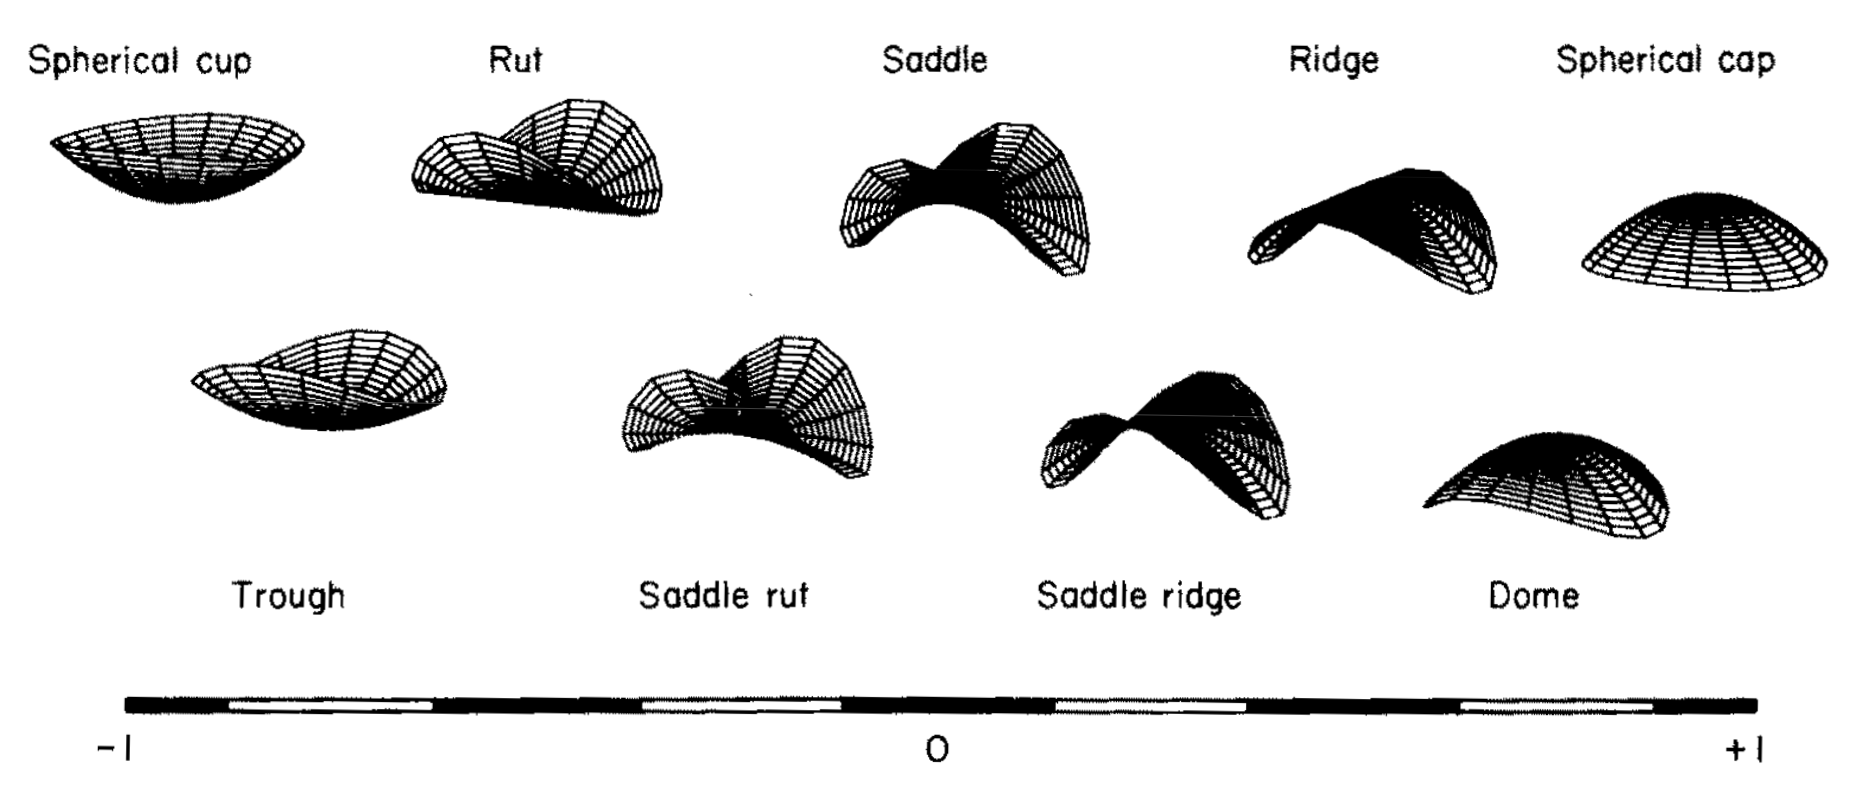
\includegraphics[width=\textwidth]{images/shape-index-range.png}
  \caption{Skala indeksu kształtu z podziałem na dziewięć kategorii. \cite{paper:shape-index}}
  \label{fig:shape-index-range}
\end{figure}

Okazało się, że na wynikowej mapie otoczenie komórek interpretowane jest jako obszar wklęsły, w przeciwieństwie do samych komórek, których wnętrze oznaczane jest indeksami kształtów wypukłych. Własność ta zachodzi na większości testowych obrazów nawet przy stosunkowo dużym zagęszczeniu komórek.

\subsection{Szkieletyzacja i wstępna detekcja komórek}

Zgodnie z powyższą obserwacją, możemy łatwo oddzielić komórkę od jej otoczenia na obrazie ustalając pewien próg $t \approx 0$. Załóżmy przez chwilę, że binaryzując w ten sposób mapę indeksów kształtu otrzymamy obraz $\image_{bin}$, na którym każdy piksel leżący wewnątrz dowolnej komórki będzie miał wartość $1$, natomiast każdy piksel należący do zewnętrznego obrysu dowolnej komórki (nie należący do komórki, lecz sąsiadujący z pikselem należącym do niej) będzie miał wartość $0$.
Przy takim założeniu każda komórka jest niezależną ,,wyspą'' na binarnym obrazie $\image_{bin}$. Chcąc odnaleźć ,,kręgosłup'' komórki (łamaną przechodzącą przez jej środek) chcemy tak naprawdę znaleźć łamaną, która jest równoodległa od jej krawędzi. Bardzo podobny problem rozwiązują algorytmy do wyznaczania szkieletu -- ich celem jest odnalezienie zbioru punktów równoodległych od co najmniej dwóch brzegów.

Na potrzeby tej pracy do szkieletonizacji użyta została implementacja algorytmu ,,3D thinning algorithm''\cite{algo:3d-thinning} w formie pluginu dla programu ImageJ\cite{plugin:skeletonize-3d}. Mimo iż wtyczka pozwala na szkieletyzację obrazów 3D, w tym przypadku została użyta do przetworzenia pojedynczego obrazu 2D. Wynikiem szkieletyzacji jest binarny obraz o pewnych właściwościach. Każdy aktywny piksel można przyporządkować do trzech grup:
\begin{itemize}
  \item końcówki -- mają mniej niż 2 sąsiadujące aktywne piksele
  \item węzły -- mają więcej niż 2 sąsiadujące aktywne piksele
  \item połączenia -- mają dokładnie 2 sąsiadujące aktywne piksele.
\end{itemize}
Przedstawiając szkielet jako graf końcówki tworzyłyby wierzchołki o stopniu równym $1$ lub $0$, wierzchołki o większych stopniach przedstawiałyby zbiory sąsiadujących ze sobą węzłów, natomiast krawędzie reprezentowałyby zbiory sąsiadujących ze sobą połączeń (zakończonych zbiorem węzłów lub końcówką). Taką reprezentację grafową można uzyskać za pomocą kolejnej wtyczki dla programu ImageJ tego samego autora\cite{plugin:analyze-skeleton}. Poza standardowymi informacjami wierzchołki i krawędzie utworzonego za jej pomocą grafu przechowują zbiory pikseli które reprezentują.

Ze względu na specyficzny kształt komórki można zaobserwować następującą właściwość: po przeprowadzeniu szkieletyzacji obrazu $\image_{bin}$, o ile przyjęte wcześniej założenie jest spełnione, szkielet każdej z komórek składa się dokładnie z dwóch końcówek i połączeń między nimi. Łamaną opisującą zbiór połączeń można z powodzeniem nazwać ,,kręgosłupem komórki''. Mając do dyspozycji zbiór punktów $\mathbf{P}$ lokalizujących komórki można teraz w łatwy sposób odnaleźć dla każdej z nich graf ją opisujący (zawierający dwa wierzchołki i jedną krawędź). Jednym ze sposobów może być wyszukanie dla każdego punktu ze zbioru $\mathbf{P}$ krawędź która znajduje się najbliżej tego punktu, gdzie odległość między punktem a krawędzią zdefiniowana jest jako odległość między punktem, a najbliższym pikselem, który należy do zbioru opisywanego przez tę krawędź.

\subsection{Wybór krawędzi w węzłach}

Niestety przyjęte założenie o tym, że każdy piksel należący do zewnętrznego obrysu dowolnej komórki będzie miał wartość $0$, nie zawsze jest spełnione. W realistycznym scenariuszu zdarza się, że jedna z końcówek komórki znajdują się na tyle blisko innej komórki, że wstępne przetwarzanie i progowanie obrazu nie powoduje ich rozdzielenia na obrazie binarnym. Czasem artefakty widoczne na obrazie wejściowym powodują, że wyspa na obrazie binarnym zawiera nie tylko komórkę, ale także fragment innego kształtu. W zdecydowanej większości takich przypadków kręgosłup komórki można opisać spójnym podgrafem o stopniu 2 grafu reprezentującego szkielet wyspy zawierającej komórki.

Wstępna detekcja kręgosłupa danej komórki polega, tak jak w scenariuszu optymistycznym, na odnalezieniu krawędzi $\{v_0, u_0\}$ w grafie $\mathbf{G}$ leżącej najbliżej punktu opisującego komórkę, a następnie na stworzeniu z niej i jej wierzchołków nowego grafu $\mathbf{S}_0$. Tak utworzony kręgosłup rozszerzany jest później zgodnie z następującym algorytmem:

\begin{algorithmic}
\FORALL{$v \gets v_0, u_0$}
  \LOOP
    \STATE
      $\text{E}_v \gets$ podzbiór krawędzi grafu $E(\mathbf{G}) - E(\mathbf{S}_n)$ incydentnych do $v$,\newline
      \hphantom{$\text{E}_v \gets$} które nie tworzą cyklu w grafie $\mathbf{S}_n$
    \IF{$\text{E}_v = \O$}
      \STATE \textbf{break}
    \ENDIF
    \STATE $\{v, u\} \gets \argmax_{e \in \text{E}_v} q_v(e)$
    \STATE $\mathbf{S}_{n+1} \gets \mathbf{S}_n \cup (\{u\}, \{\{v, u\}\}) $
    \STATE $v \gets u$
  \ENDLOOP
\ENDFOR
\end{algorithmic}
gdzie funkcja $q_v(e)$ jest funkcją oceny, która służy do wyboru najmocniej związanej krawędzi. Siła wiązania zdefiniowana jest tutaj jako najniższa wartość indeksu kształtu (oryginalnego obrazu) dla piksela leżącego na krawędzi $e$, w okolicy wierzchołka $v$ (w odległości nie większej niż pewna stała $d$ od środka masy pikseli tworzących węzeł $v$).

Takie rozwiązanie sprawdza się dobrze dla komórek, których kręgosłup znajduje się w grafie $\mathbf{G}$, oraz jego zakończenia w tym grafie mają stopień $1$. Pomijam na ten moment przypadek, gdy szukany kręgosłup komórki nie istnieje w grafie $\mathbf{G}$. W pozostałych przypadkach przynajmniej jedno z zakończeń szukanego kręgosłupa $\mathbf{S}$ ma w grafie $\mathbf{G}$ stopień większy niż $1$. Zatem, o ile funkcja oceny $q_v(e)$ sprawdzi się dobrze jeśli chodzi o dobór krawędzi należących do szukanego kręgosłupa komórki, uzyskany na końcu algorytmu kręgosłup $\mathbf{S}_n$ będzie nadgrafem szukanego kręgosłupa $\mathbf{S}$. W takim przypadku ,,nadmiarowa'' część kręgosłupa należy do szkieletu innej komórki lub jest wynikiem artefaktu widocznego na oryginalnym obrazie. Drugi przypadek pozostawiam do ręcznego rozwiązania użytkownikowi. Pierwszy natomiast, nachodzące na siebie kręgosłupy komórek, rozwiązuję automatycznie.

\subsection{Rozwiązywanie konfliktów}

Rozdzielanie nachodzących na siebie komórek nazwałem ,,rozwiązywaniem konfliktów''. Niech $\mathbf{\Sigma}_0$ będzie zbiorem wszystkich znalezionych kręgosłupów, natomiast $X(\mathbf{\Sigma})$ zbiorem par kręgosłupów nachodzących na siebie należących do zbioru $\mathbf{\Sigma}$. Rozwiązywanie konfliktów przebiega następująco:

\begin{algorithmic}

\WHILE{$X(\mathbf{\Sigma}_n) \neq \O$}
  \STATE $\{S_x, S_y\} \gets$ dowolna para ze zbioru $X(\mathbf{\Sigma})$
  \STATE $\{S_x', S_y'\} \gets$ rozwiąż konflikt pomiędzy $S_x$ i $S_y$
  \STATE $\mathbf{\Sigma}_{n+1} \gets (\mathbf{\Sigma}_n - \{S_x, S_y\}) \cup \{S_x', S_y'\}$
\ENDWHILE

\end{algorithmic}


\subsection{Uzyskiwanie linii łamanej}

\ldots % TODO Uzyskiwanie linii łamanej


\subsection{Korekta końcówek}

\ldots % TODO Poprawianie końcówek (dociąganie do krawędzi)


\section{Śledzenie komórek w czasie}
\label{sec:cell-tracking}

\ldots % TODO Śledzenie komórek w czasie

% Opis jednej iteracji + sprawdzenia czy komórka nie powinna zostać podzielona

\section{Interakcja ze strony użytkownika}

\ldots % TODO Interakcja ze strony użytkownika


%%%%%%%%%%%%%%%%%%%%%%%%%%%%%%%%%%%%%%%%%%%%%%%%%%%%%%%%%%%%%%%%%%%%%%%%%%%%%%%%%%%%%%%%%%%

\chapter{Opis implementacji}

\section{Kod źródłowy}
\ldots % TODO Kod źródłowy
\section{Kompilacja i uruchomienie}
\ldots % TODO Kod źródłowy
\section{Struktury danych}
\ldots % TODO Struktury danych
\section{Architektura}
\ldots % TODO Architektura
\section{Opis wykorzystanego API ImageJ}
\ldots % TODO Opis wykorzystanego API ImageJ
\section{Błędy w implementacji ImageJ i sposoby na ich obejście}
\ldots % TODO Błędy w implementacji ImageJ i sposoby na ich obejście
\section{Opis sposobu dalszego rozwoju, interfejsy}
\ldots % TODO Opis sposobu dalszego rozwoju, interfejsy




%%%%%%%%%%%%%%%%%%%%%%%%%%%%%%%%%%%%%%%%%%%%%%%%%%%%%%%%%%%%%%%%%%%%%%%%%%%%%%%%%%%%%%%%%%%

\chapter{Zakończenie}

\section{Podsumowanie}
\ldots % TODO Podsumowanie
\section{Ograniczenia wynikające z zastosowanych metod}
\ldots % TODO Ograniczenia wynikające z zastosowanych metod
\section{Dalszy rozwój}
\ldots % TODO Dalszy rozwój




%%%%% BIBLIOGRAFIA


%\bibitem{example} \ldots

\begin{thebibliography}{1}

\bibitem{paper:shape-index}
  Jan J Koenderink, Andrea J van Doorn,
  \emph{Surface shape and curvature scales},
  Image and Vision Computing,
  10:557–565,
  1992.

\bibitem{plugin:shape-index-map}
  Johannes Schindelin,
  \emph{Shape Index Map},
  2010,
  \url{https://imagej.net/Shape_Index_Map}.

\bibitem{algo:3d-thinning}
  Ta-Chih Lee, Rangasami L. Kashyap, Chong-Nam Chu,
  \emph{Building skeleton models via 3-D medial surface/axis thinning algorithms},
  Computer Vision, Graphics, and Image Processing,
  56(6):462–478,
  1994.

\bibitem{plugin:skeletonize-3d}
  Ignacio Arganda-Carreras,
  \emph{Skeletonize3D},
  2.1.1,
  2017,
  \url{https://imagej.net/Skeletonize3D}.

\bibitem{plugin:analyze-skeleton}
  Ignacio Arganda-Carreras,
  \emph{AnalyzeSkeleton},
  3.3.0,
  2018,
  \url{https://imagej.net/AnalyzeSkeleton}.

\end{thebibliography}

\end{document}
